\documentclass[tikz]{standalone}
\usepackage{amsmath, amssymb, amsfonts}
\usetikzlibrary {arrows.meta}
\usetikzlibrary {calc}
\begin{document}
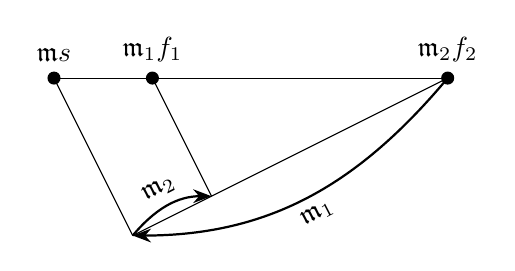
\begin{tikzpicture}[>=Stealth,
        point/.style={circle, fill=black, minimum size=1pt, scale=0.5}]
    \coordinate (s) at (0, 0);
    \coordinate (f2) at (5, 0);
    \coordinate (h) at (1, -2);
    \coordinate (f1) at ($(s)!0.25!(f2)$);
    \coordinate (hs) at ($(h)!0.25!(f2)$);

    \draw (s) -- (f2);
    \draw (h) -- (f2);
    \draw (h) -- (s);
    \draw (hs) -- (f1);

    \node[point, label=$\mathfrak{m}_1f_1$] at (f1) {};
    \node[point, label=$\mathfrak{m}_2f_2$] at (f2) {};
    \node[point, label=$\mathfrak{m}s$] at (s) {};

    \draw [->, thick] (f2) to [out=230, in=0]
    node [below, sloped]  (m1) {$\mathfrak{m}_1$} (h);
    \draw [->, thick] (h) to [out=50, in=180]
    node [above, sloped]  (m1) {$\mathfrak{m}_2$} (hs);
\end{tikzpicture}
\end{document}
